\documentclass{extbook}[14pt]
\usepackage{multicol, enumerate, enumitem, hyperref, color, soul, setspace, parskip, fancyhdr, amssymb, amsthm, amsmath, bbm, latexsym, units, mathtools}
\everymath{\displaystyle}
\usepackage[headsep=0.5cm,headheight=0cm, left=1 in,right= 1 in,top= 1 in,bottom= 1 in]{geometry}
\usepackage{dashrule}  % Package to use the command below to create lines between items
\newcommand{\litem}[1]{\item #1

\rule{\textwidth}{0.4pt}}
\pagestyle{fancy}
\lhead{}
\chead{Answer Key for Makeup Progress Quiz 1 Version A}
\rhead{}
\lfoot{6018-3080}
\cfoot{}
\rfoot{Spring 2021}
\begin{document}
\textbf{This key should allow you to understand why you choose the option you did (beyond just getting a question right or wrong). \href{https://xronos.clas.ufl.edu/mac1105spring2020/courseDescriptionAndMisc/Exams/LearningFromResults}{More instructions on how to use this key can be found here}.}

\textbf{If you have a suggestion to make the keys better, \href{https://forms.gle/CZkbZmPbC9XALEE88}{please fill out the short survey here}.}

\textit{Note: This key is auto-generated and may contain issues and/or errors. The keys are reviewed after each exam to ensure grading is done accurately. If there are issues (like duplicate options), they are noted in the offline gradebook. The keys are a work-in-progress to give students as many resources to improve as possible.}

\rule{\textwidth}{0.4pt}

\begin{enumerate}\litem{
Determine the domain of the function below.
\[ f(x) = \frac{6}{9x^{2} +3 x -20} \]The solution is \( \text{All Real numbers except } x = -1.667 \text{ and } x = 1.333. \), which is option B.\begin{enumerate}[label=\Alph*.]
\item \( \text{All Real numbers except } x = a \text{ and } x = b, \text{ where } a \in [-16, -14] \text{ and } b \in [12, 14] \)

All Real numbers except $x = -15.000$ and $x = 12.000$, which corresponds to not factoring the denominator correctly.
\item \( \text{All Real numbers except } x = a \text{ and } x = b, \text{ where } a \in [-3.67, 0.33] \text{ and } b \in [1.33, 5.33] \)

All Real numbers except $x = -1.667$ and $x = 1.333$, which is the correct option.
\item \( \text{All Real numbers.} \)

This corresponds to thinking the denominator has complex roots or that rational functions have a domain of all Real numbers.
\item \( \text{All Real numbers except } x = a, \text{ where } a \in [-16, -14] \)

All Real numbers except $x = -15.000$, which corresponds to removing a distractor value from the denominator.
\item \( \text{All Real numbers except } x = a, \text{ where } a \in [-3.67, 0.33] \)

All Real numbers except $x = -1.667$, which corresponds to removing only 1 value from the denominator.
\end{enumerate}

\textbf{General Comment:} Recall that dividing by zero is not a real number. Therefore the domain is all real numbers \textbf{except} those that make the denominator 0.
}
\litem{
Solve the rational equation below. Then, choose the interval(s) that the solution(s) belongs to.
\[ \frac{-2x}{-7x + 6} + \frac{-6x^{2}}{28x^{2} +25 x -42} = \frac{-4}{-4x -7} \]The solution is \( \text{There are two solutions: } x = 3.000 \text{ and } x = 4.000 \), which is option E.\begin{enumerate}[label=\Alph*.]
\item \( x \in [3.5,7.7] \)


\item \( x_1 \in [2.5, 3.8] \text{ and } x_2 \in [-1.14,3.86] \)


\item \( \text{All solutions lead to invalid or complex values in the equation.} \)


\item \( x \in [-4.1,0.9] \)


\item \( x_1 \in [2.5, 3.8] \text{ and } x_2 \in [2,9] \)

* $x = 3.000 \text{ and } x = 4.000$, which is the correct option.
\end{enumerate}

\textbf{General Comment:} Distractors are different based on the number of solutions. Remember that after solving, we need to make sure our solution does not make the original equation divide by zero!
}
\litem{
Choose the graph of the equation below.
\[ f(x) = \frac{-1}{(x + 3)^2} + 1 \]The solution is the graph below, which is option A.
\begin{center}
    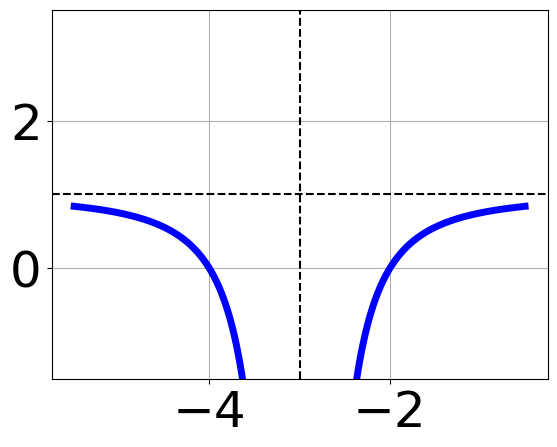
\includegraphics[width=0.3\textwidth]{../Figures/rationalEquationToGraphCopyAA.png}
\end{center}\begin{enumerate}[label=\Alph*.]
\begin{multicols}{2}
\item 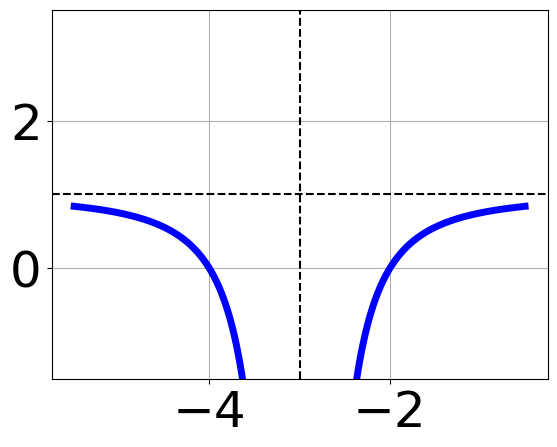
\includegraphics[width = 0.3\textwidth]{../Figures/rationalEquationToGraphCopyAA.png}
\item 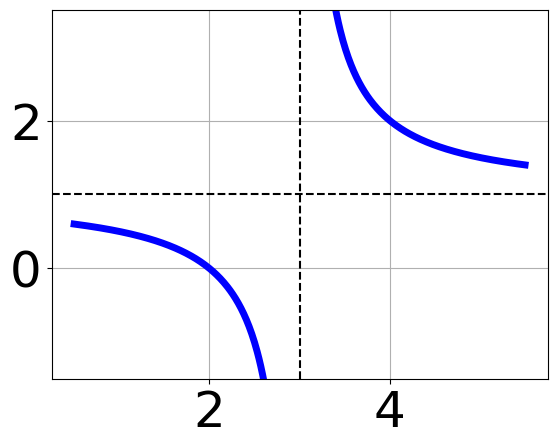
\includegraphics[width = 0.3\textwidth]{../Figures/rationalEquationToGraphCopyBA.png}
\item 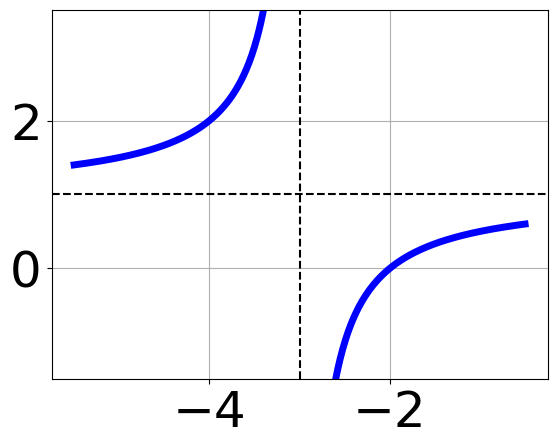
\includegraphics[width = 0.3\textwidth]{../Figures/rationalEquationToGraphCopyCA.png}
\item 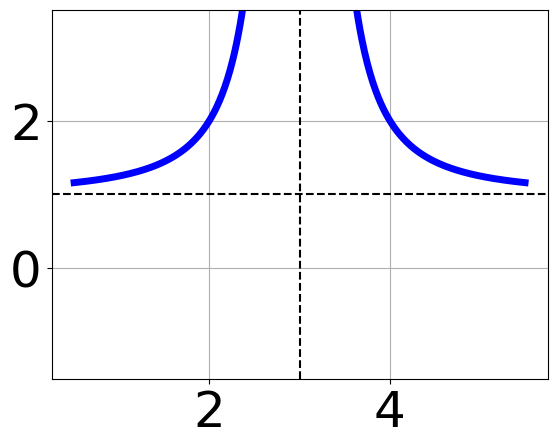
\includegraphics[width = 0.3\textwidth]{../Figures/rationalEquationToGraphCopyDA.png}
\end{multicols}\item None of the above.\end{enumerate}
\textbf{General Comment:} Remember that the general form of a basic rational equation is $ f(x) = \frac{a}{(x-h)^n} + k$, where $a$ is the leading coefficient (and in this case, we assume is either $1$ or $-1$), $n$ is the degree (in this case, either $1$ or $2$), and $(h, k)$ is the intersection of the asymptotes.
}
\litem{
Choose the graph of the equation below.
\[ f(x) = \frac{1}{x + 3} - 2 \]The solution is the graph below, which is option E.
\begin{center}
    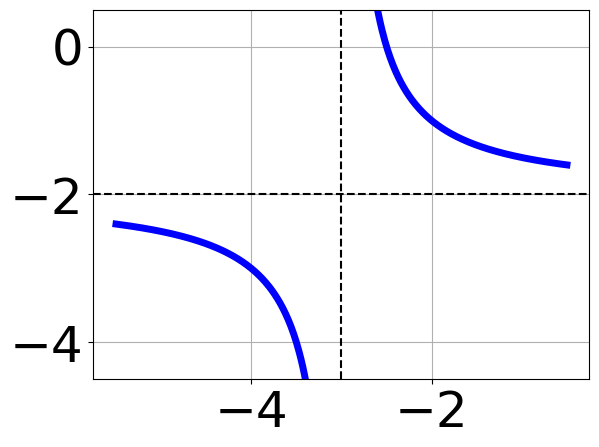
\includegraphics[width=0.3\textwidth]{../Figures/rationalEquationToGraphEA.png}
\end{center}\begin{enumerate}[label=\Alph*.]
\begin{multicols}{2}
\item 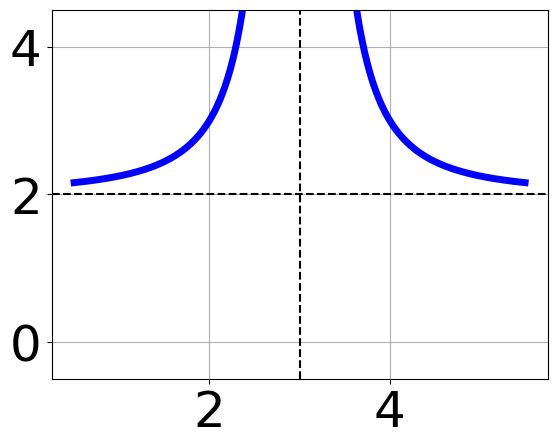
\includegraphics[width = 0.3\textwidth]{../Figures/rationalEquationToGraphAA.png}
\item 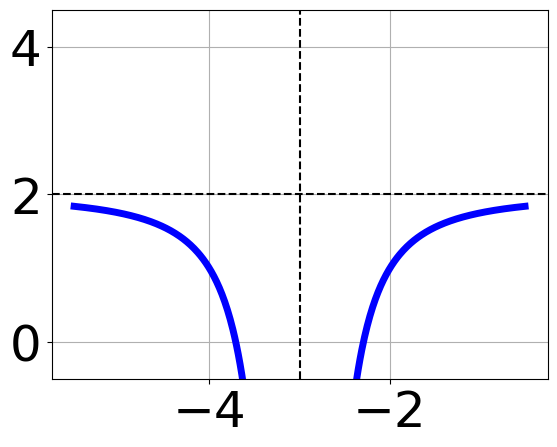
\includegraphics[width = 0.3\textwidth]{../Figures/rationalEquationToGraphBA.png}
\item 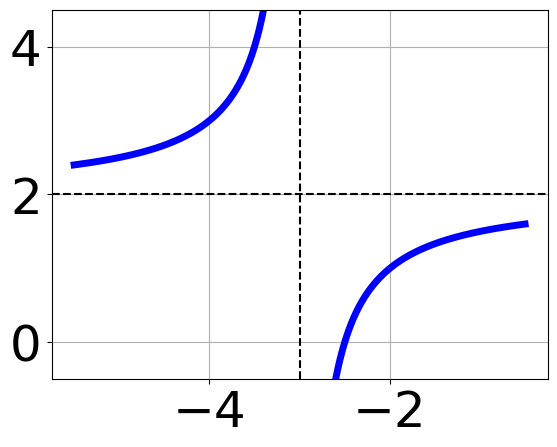
\includegraphics[width = 0.3\textwidth]{../Figures/rationalEquationToGraphCA.png}
\item 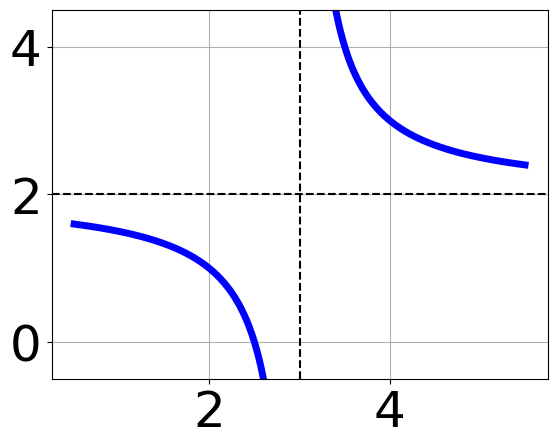
\includegraphics[width = 0.3\textwidth]{../Figures/rationalEquationToGraphDA.png}
\end{multicols}\item None of the above.\end{enumerate}
\textbf{General Comment:} Remember that the general form of a basic rational equation is $ f(x) = \frac{a}{(x-h)^n} + k$, where $a$ is the leading coefficient (and in this case, we assume is either $1$ or $-1$), $n$ is the degree (in this case, either $1$ or $2$), and $(h, k)$ is the intersection of the asymptotes.
}
\litem{
Choose the equation of the function graphed below.

\begin{center}
    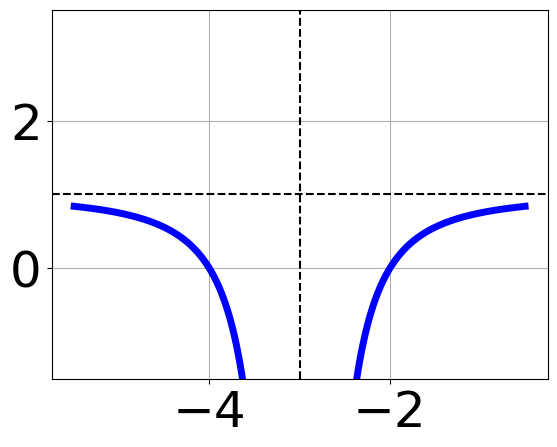
\includegraphics[width=0.5\textwidth]{../Figures/rationalGraphToEquationCopyA.png}
\end{center}


The solution is \( \text{None of the above as it should be } f(x) = \frac{-1}{(x + 3)^2} + 1 \), which is option E.\begin{enumerate}[label=\Alph*.]
\item \( f(x) = \frac{1}{(x + 3)^2} - 2 \)

Corresponds to using the general form $f(x) = \frac{a}{(x-h)^2}+k$, the opposite leading coefficient, AND not noticing the $y$-value was wrong.
\item \( f(x) = \frac{1}{x + 3} - 2 \)

Corresponds to thinking the graph was a shifted version of $\frac{1}{x}$, using the general form $f(x) = \frac{a}{(x-h)^2}+k$, the opposite leading coefficient, AND not noticing the $y$-value was wrong.
\item \( f(x) = \frac{-1}{x - 3} - 2 \)

Corresponds to thinking the graph was a shifted version of $\frac{1}{x}$ AND not noticing the $y$-value was wrong.
\item \( f(x) = \frac{-1}{(x - 3)^2} - 2 \)

The $x$- and $y$-value of the equation does not match the graph.
\item \( \text{None of the above} \)

None of the equation options were the correct equation.
\end{enumerate}

\textbf{General Comment:} Remember that the general form of a basic rational equation is $ f(x) = \frac{a}{(x-h)^n} + k$, where $a$ is the leading coefficient (and in this case, we assume is either $1$ or $-1$), $n$ is the degree (in this case, either $1$ or $2$), and $(h, k)$ is the intersection of the asymptotes.
}
\litem{
Solve the rational equation below. Then, choose the interval(s) that the solution(s) belongs to.
\[ \frac{-4x}{3x + 7} + \frac{-6x^{2}}{-15x^{2} -23 x + 28} = \frac{6}{-5x + 4} \]The solution is \( \text{There are two solutions: } x = -0.901 \text{ and } x = 3.330 \), which is option E.\begin{enumerate}[label=\Alph*.]
\item \( x_1 \in [-5.8, 0.2] \text{ and } x_2 \in [-5.33,0.67] \)


\item \( x \in [1.7,6.1] \)


\item \( x \in [-0.1,2.2] \)


\item \( \text{All solutions lead to invalid or complex values in the equation.} \)


\item \( x_1 \in [-5.8, 0.2] \text{ and } x_2 \in [2.33,12.33] \)

* $x = -0.901 \text{ and } x = 3.330$, which is the correct option.
\end{enumerate}

\textbf{General Comment:} Distractors are different based on the number of solutions. Remember that after solving, we need to make sure our solution does not make the original equation divide by zero!
}
\litem{
Determine the domain of the function below.
\[ f(x) = \frac{5}{36x^{2} +54 x + 18} \]The solution is \( \text{All Real numbers except } x = -1.000 \text{ and } x = -0.500. \), which is option E.\begin{enumerate}[label=\Alph*.]
\item \( \text{All Real numbers except } x = a, \text{ where } a \in [-36.22, -34.75] \)

All Real numbers except $x = -36.000$, which corresponds to removing a distractor value from the denominator.
\item \( \text{All Real numbers except } x = a, \text{ where } a \in [-2.17, -0.85] \)

All Real numbers except $x = -1.000$, which corresponds to removing only 1 value from the denominator.
\item \( \text{All Real numbers.} \)

This corresponds to thinking the denominator has complex roots or that rational functions have a domain of all Real numbers.
\item \( \text{All Real numbers except } x = a \text{ and } x = b, \text{ where } a \in [-36.22, -34.75] \text{ and } b \in [-18.97, -17.51] \)

All Real numbers except $x = -36.000$ and $x = -18.000$, which corresponds to not factoring the denominator correctly.
\item \( \text{All Real numbers except } x = a \text{ and } x = b, \text{ where } a \in [-2.17, -0.85] \text{ and } b \in [-0.79, -0.36] \)

All Real numbers except $x = -1.000$ and $x = -0.500$, which is the correct option.
\end{enumerate}

\textbf{General Comment:} Recall that dividing by zero is not a real number. Therefore the domain is all real numbers \textbf{except} those that make the denominator 0.
}
\litem{
Choose the equation of the function graphed below.

\begin{center}
    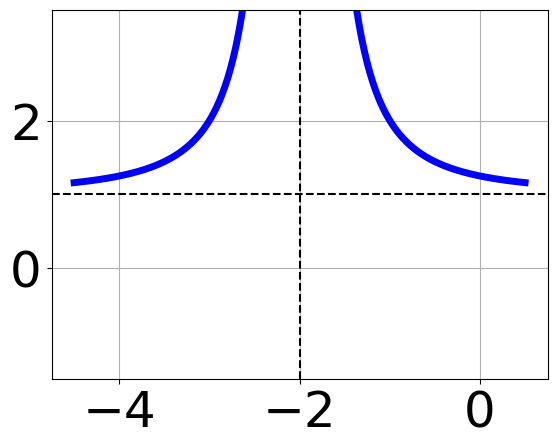
\includegraphics[width=0.5\textwidth]{../Figures/rationalGraphToEquationA.png}
\end{center}


The solution is \( \text{None of the above as it should be } f(x) = \frac{1}{(x + 2)^2} + 1 \), which is option E.\begin{enumerate}[label=\Alph*.]
\item \( f(x) = \frac{1}{(x - 2)^2} + 1 \)

The $x$-value of the equation does not match the graph.
\item \( f(x) = \frac{1}{x - 2} + 1 \)

Corresponds to thinking the graph was a shifted version of $\frac{1}{x}$.
\item \( f(x) = \frac{-1}{(x + 2)^2} + 1 \)

Corresponds to using the general form $f(x) = \frac{a}{(x-h)^2}+k$ and the opposite leading coefficient.
\item \( f(x) = \frac{-1}{x + 2} + 1 \)

Corresponds to thinking the graph was a shifted version of $\frac{1}{x}$, using the general form $f(x) = \frac{a}{(x-h)^2}+k$, and the opposite leading coefficient.
\item \( \text{None of the above} \)

None of the equation options were the correct equation.
\end{enumerate}

\textbf{General Comment:} Remember that the general form of a basic rational equation is $ f(x) = \frac{a}{(x-h)^n} + k$, where $a$ is the leading coefficient (and in this case, we assume is either $1$ or $-1$), $n$ is the degree (in this case, either $1$ or $2$), and $(h, k)$ is the intersection of the asymptotes.
}
\litem{
Solve the rational equation below. Then, choose the interval(s) that the solution(s) belongs to.
\[ \frac{-6}{-4x -9} + 6 = \frac{5}{20x + 45} \]The solution is \( x = -2.458 \), which is option B.\begin{enumerate}[label=\Alph*.]
\item \( x \in [0.9,4.1] \)

$x = 2.042$, which corresponds to not distributing the factor $-4x -9$ correctly when trying to eliminate the fraction.
\item \( x \in [-3.46,-1.46] \)

* $x = -2.458$, which is the correct option.
\item \( x_1 \in [-4.1, -2.7] \text{ and } x_2 \in [-2.46,-0.46] \)

$x = -2.708 \text{ and } x = -2.458$, which corresponds to getting the correct solution and believing there should be a second solution to the equation.
\item \( x_1 \in [-2.6, -2.4] \text{ and } x_2 \in [0.04,3.04] \)

$x = -2.458 \text{ and } x = 2.042$, which corresponds to getting the correct solution and believing there should be a second solution to the equation.
\item \( \text{All solutions lead to invalid or complex values in the equation.} \)

This corresponds to thinking $x = -2.458$ leads to dividing by zero in the original equation, which it does not.
\end{enumerate}

\textbf{General Comment:} Distractors are different based on the number of solutions. Remember that after solving, we need to make sure our solution does not make the original equation divide by zero!
}
\litem{
Solve the rational equation below. Then, choose the interval(s) that the solution(s) belongs to.
\[ \frac{3}{-4x + 8} + -2 = \frac{-4}{-32x + 64} \]The solution is \( x = 1.562 \), which is option A.\begin{enumerate}[label=\Alph*.]
\item \( x \in [1.56,2.56] \)

* $x = 1.562$, which is the correct option.
\item \( x_1 \in [0.5, 1.31] \text{ and } x_2 \in [1.56,3.56] \)

$x = 1.125 \text{ and } x = 1.562$, which corresponds to getting the correct solution and believing there should be a second solution to the equation.
\item \( x_1 \in [-2.7, -1.89] \text{ and } x_2 \in [1.56,3.56] \)

$x = -2.438 \text{ and } x = 1.562$, which corresponds to getting the correct solution and believing there should be a second solution to the equation.
\item \( x \in [-2.7,-1.89] \)

$x = -2.438$, which corresponds to not distributing the factor $-4x + 8$ correctly when trying to eliminate the fraction.
\item \( \text{All solutions lead to invalid or complex values in the equation.} \)

This corresponds to thinking $x = 1.562$ leads to dividing by zero in the original equation, which it does not.
\end{enumerate}

\textbf{General Comment:} Distractors are different based on the number of solutions. Remember that after solving, we need to make sure our solution does not make the original equation divide by zero!
}
\end{enumerate}

\end{document}